\documentclass[11pt]{amsart}
\usepackage[margin=1in, marginparwidth=0.8in]{geometry}
\usepackage[colorlinks,linkcolor=black!50!red,citecolor=blue,pdfpagemode=None]{hyperref}
\usepackage[capitalise]{cleveref}
\usepackage{graphicx}

\usepackage[draft]{say}
\newcommand{\saySS}[1]{\say[SS]{#1}}

% shorthands 
\newcommand{\cA}{\mathcal{A}}
\newcommand{\bC}{\mathbb{C}}
\newcommand{\cAb}{\mathcal{A}_\bullet}
\newcommand{\Supp}{\operatorname{Supp}}
\newcommand{\ZZ}{\mathbb{Z}}
\newcommand{\bg}{\mathbf{g}}
\newcommand{\bc}{\mathbf{c}}
\newcommand{\bb}{\mathbf{b}}

% ambients and numbering
\newtheorem{theorem}{Theorem}[section]
\newtheorem{conjecture}[theorem]{Conjecture}
\newtheorem{corollary}[theorem]{Corollary}
\newtheorem{definition}[theorem]{Definition}
\newtheorem{lemma}[theorem]{Lemma}
\newtheorem{proposition}[theorem]{Proposition}
\newtheorem{example}[theorem]{Example}
\newtheorem{remark}[theorem]{Remark}
\numberwithin{equation}{section}

\begin{document}
\title[Exchange relations for finite type]{Exchange relations for finitie type cluster algebras with acyclic initial seed and principal coefficients}

\author[Felikson]{Anna Felikson}
\address[Anna Felikson]{Durham University}
\email{email-here}

\author[Reading]{Nathan Reading}
\address[Nathan Reading]{North Carolina State Univesity}
\email{email-here}

\author[Stella]{Salvatore Stella}
\address[Salvatore Stella]{IN$d$AM - Marie Curie Actions fellow, Universit\`a\`{ }La Sapienza'', Roma, Italy.}
\email{stella@mat.uniroma1.it}

\author[tumarkin]{Pavel Tumarkin}
\address[Pavel Tumarkin]{Durham University}
\email{email-here}

\begin{abstract}
We give an explicit description of all the exchange relations for finitie type cluster algebras with acyclic initial seed and principal coefficients.
\end{abstract}

\maketitle

\section{Introduction}
  In \cite{Ste13} the third author gave a formula for all the exchange relations in any finite type acyclic cluster algebra without coefficients.
  Our main theorem here improves on this result to deal with principal coefficients.
  
  \begin{theorem}
    \label{thm:main_vague}
    In any cluster algebra of finite type with principal coefficients at an acyclic initial seed, the coefficient appearing in the exchange relation of any two exchangeable cluster variables is \emph{explicitly} determined by their $\bg$-vectors. 
  \end{theorem}
  
  The claim in previous statement lays in the word ``explicitly''. 
  Indeed, since cluster variables are parametrized by their $\bg$-vectors, and since exchange relations are prescribed by the cluster variables involved, it is obvious that the $\bg$-vectors determines indirectly the coefficients. 
  This note is about giving precise formulas to compute them.
 
  In order to make \cref{thm:main_vague} more precise we need to recall few notions and results from \cite{Ste13,YZ08}.

  Let $A$ be any finite type \emph{Cartan matrix} and denote by $W=\langle s_1,\dots,s_n\rangle$ the associated \emph{Weyl group} and \emph{simple reflections}.
  To each \emph{Coxeter element} $c=s_{i_1}\cdots s_{i_n}$ in $W$ we can associate a skew-symmetrizable integer matrix $B_c=(b_{ij})_{i,j\in[1,n]}$ by setting
  \[
    b_{ij}=
    \begin{cases}
      -a_{ij} & \text{if } i\prec_c j  \\
      a_{ij}  & \text{if } j\prec_c i  \\
      0       & \text{otherwise}
    \end{cases}
  \]
  where we write $i\prec_c j$ if and only if $s_i$ precedes $s_j$ in all reduced expressions of $c$.
  As $c$ varies we get all the possible \emph{acyclic} exchange matrices in any cluster algebra of the same type as $A$.
  We will denote by $\cA(c)$ (resp. $\cA_0(c)$) the cluster algebra with initial exchange matrix $B_c$ and  \emph{principal} (resp. \emph{without}) \emph{coefficients} at the initial seed.

  The algebra $\cA(c)$ is $\ZZ^n$-graded; its cluster variables and cluster monomials are homogeneous elements and their \emph{$\bg$-vector} is their homogeneous degree.
  Let $\omega_i$ be the i-th \emph{fundamental weight} in the \emph{weight lattice} $P$ of $A$; we will routinely identify $\ZZ^n$ with $P$ by means of the basis of fundamental weights.
  We will therefore always consider $\bg$-vectors as elements of $P$.

  Let $w_0$ be the longest element of $W$ and denote by $h(i;c)$ the minimum positive integer such that 
  \[
    c^{h(i;c)}\omega_i = w_0\omega_i
  \]
  (it is a finite number \cite[Proposition 1.3]{YZ08}).
  \begin{theorem}[{\cite[Theorem 1.4]{YZ08}}]
    The cluster variables of $\cA(c)$ are naturally in bijection with the elements of the set
    \[
      \Pi(c)
      :=
      \left\{
        c^m\omega_i \, :\, i\in[1,n] \, , \, 0\leq m \leq h(i;c) 
      \right\}.
    \]
    To the cluster variable $x_\lambda$ it corresponds its $\bg$-vector $\lambda\in\Pi(c)$.
  \end{theorem}
  This correspondence extends to a bijection between points of $P$ and \emph{cluster monomials} of $\cA(c)$ (cf. \cite[Theorem 1.2]{Ste13}); for $\lambda\in P$ we will denote by $x_\lambda$ the cluster monomial whose $\bg$-vector is $\lambda$.
  In view of the ``separation of additions formula'' we get a similar bijection with cluster monomials in $\cA_0(c)$; we will freely refer to either of the two according to our needs.

  The set $\Pi(c)$ is naturally endowed with a permutation $\tau_c$ defined by
  \[
    \tau_c (\lambda) 
    :=
    \begin{cases}
      \omega_i  & \text{if $\lambda = -\omega_i$} \\
      c\lambda  & \text{otherwise}
    \end{cases}
  \]
  which extends to a piecewise linear map on the whole of $P$ compatible with the cluster structure of $\cA(c)$.
  This is a combinatorial shadow of a notable automorphism of $\cA_0(c)$ sending $x_\lambda$ to $x_{\tau_c(\lambda)}$. 

  Let $Q$ be the \emph{root lattice} of $A$ with simple roots $\alpha_i$; as for $P$, we will identify $Q$ and $\ZZ^n$ using the basis of simple roots.
  \begin{definition}
    The \emph{compatibility degree} $(\bullet||\bullet)_c$ is the unique $\tau_c$-invariant function on pairs of elements of $\Pi(c)$ defined by the initial conditions
    \[
      (\omega_i||\lambda)_c
      :=
      \left[ (c^{-1}-1)\lambda ; \alpha_i\right]_+
    \]
    where $[v,\alpha_i]$ is the coefficient of $\alpha_i$ in $v$ expressed in the basis of simple roots and $[m]_+$  denotes $\max\{m, 0\}$ (cf. \cite[Proposition 5.1]{YZ08}).
  \end{definition}
  The name comes from the following important property.
  \begin{proposition}
    Two weights $\lambda$ and $\mu$ from $\Pi(c)$ are
    \begin{itemize}
      \item
        \emph{compatible} (i.e. there is a cluster of $\cA(c)$ containing both $x_\lambda$ and $x_\mu$) if and only if
        \[
          (\lambda||\mu)_c = 0
          \quad \quad
          \text{(equivalently $(\mu||\lambda)_c=0$)}
        \]

      \item
        \emph{exchangeable} (i.e. there are two clusters of $\cA(c)$ that can be obtained from one-another by swapping $x_\lambda$ for $x_\mu$) if and only if
        \[
          (\lambda||\mu)_c = 1 = (\mu||\lambda)_c
        \]
    \end{itemize}
  \end{proposition}

  Our starting point is the following restatement of \cite[Propositions 5.1 and 5.2]{Ste13}. 
  \begin{proposition}
    Suppose $\lambda$ and $\mu$ are exchangeable weights in $\Pi(c)$. 
    Then the set
    \[
      \left\{
        \tau_c^{-m}\left(\tau_c^m(\lambda)+\tau_c^m(\mu)\right)
      \right\}_{m\in\ZZ}
    \]
    consists precisely of two elements. One of them is $\lambda+\mu$; denote the other by $\lambda\uplus_c\mu$.

    The exchange relation of $x_\lambda$ and $x_\mu$ in $\cA_0(c)$ is then
    \[
      x_\lambda x_\mu = x_{\lambda+\mu} + x_{\lambda\uplus_c\mu}.
    \]
  \end{proposition}

  Denote by $y_1,\dots,y_n$ the generators of the coefficient semifield of $\cA(c)$ and by $y^\alpha$ the product $\prod_{i=1}^n y_i^{[\alpha;\alpha_i]}$.
  In view of \cite{NS14}, taking into account that the exchange relations in $\cA(c)$ are homogeneous, we get the following straightforward corollary.
  \begin{corollary}
    The exchange relations in $\cA(c)$ are all of the form 
    \[
      x_\lambda x_\mu = x_{\lambda+\mu} + y^\alpha x_{\lambda\uplus_c\mu}
    \]
    for some exchangeable weights $\lambda$ and $\mu$ and some positive root $\alpha$.
  \end{corollary}

  We can finally recast \cref{thm:main_vague} into a more precise statement.
  \begin{theorem}
    \label{thm:main}
    Let $\lambda$ and $\mu$ be exchangeable weights. 
    Then the exponent $\alpha$ in the exchange relation
    \[
      x_\lambda x_\mu = x_{\lambda+\mu} + y^\alpha x_{\lambda\uplus_c\mu}
    \]
    is the unique positive root satisfying both
    \saySS{Check signs here}
    \begin{equation}
      \label{eq:system}
      -B_c\alpha = \lambda+\mu-\lambda\uplus_c\mu
    \end{equation}
    and
    \begin{equation}
      \label{eq:dual}
      \lambda(\alpha^\vee) \mu(\alpha^\vee) = -1
    \end{equation}
    where $\alpha^\vee$ is the \emph{coroot} corresponding to $\alpha$.
  \end{theorem}
  Observe that the two conditions of the theorem are necessary. 
  Indeed \cref{eq:system} is just a restatement of the fact that the exchange relations in $\cA(c)$ are homogeneous and that the degree of $y_i$ is $-\bb_i$ (the negative of the i-th column of $B_c$).
  \cref{eq:dual}, instead, follows immediately from \cite[Eq. (1.11)]{NZ11} once we interpret $\bg$-vectors as weights and $\bc$-vectors as roots together with the observation that, mutating in direction $k$, the $k$-th $\bc$-vector changes into its negative.
  
  On the other hand \cref{eq:system} is not, in principle, sufficient on its own because $B_c$ is, in general, not invertible.
  None the less, thanks to the fact that we are dealing with positive roots, we will see that it is still enough in every case except in type $D_n$.
  
  
\section{Proof of \cref{thm:main}}
  Recall the notation for $A$, $c$ and $B_c$ from the introduction. 
  Without loss of generality we consider only Cartan matrices that are not block-decomposable.
  Further, we assume that the nodes of the Dynkin diagram of $A$ are labeled according to the standard conventions as, for example, in \cite[Table Fin]{Kac90}.

  We begin our analysis with a well known consideration on the rank of $B_c$ 
  \begin{lemma}
    \label{lem:dimensions}
    If the type of $A$ is not $D_n$, then the kernel of $B_c$ has dimension $0$ if $n$ is even and $1$ if $n$ is odd.
    If the type of $A$ is $D_n$, then the kernel of $B_c$ has dimension $2$ if $n$ is even and $1$ if $n$ is odd.
  \end{lemma}
  \begin{proof}
    The rank of $B_c$ is invariant under mutation so it suffices to establish the property for a single choice of $c$. 
    Let then $c=s_1\cdots s_n$ so that $B_c$ has positive entries above the diagonal.
    Exceptional types could be dealt uniformly in the argument at the expense of an heavier notation. 
    We prefer to check the lemma by direct inspection in those cases.

    Assume at first that the type of $A$ is not $D_n$.
    When $n$ is even, the matrix $B_c$ is invertible. 
    Indeed, expanding by the first column and then by the first row, we get:
    \[
      \det(B_c)=-\det(B_c')
    \]
    where $B_c'$ is a $(n-2)\times(n-2)$ matrix in the same infinite class of $B_c$. 
    The result follows then immediately by induction because all $2\times2$ skew-symmetrizable non-zero matrices are invertible.
    The same argument, with $n=3$ as base of the induction, shows that when $n$ is odd $\det(B_c)=0$.
    Combining the two assertions we get that, for odd $n$, the dimension of the kernel of $B_c$ is $1$.

    To get the result in type $D_n$ it is enough to observe that the last two rows (and columns) of $B_c$ are identical. 
    We deduce therefore the required property from type $A_{n-1}$.
  \end{proof}

  This establishes \cref{thm:main} whenever $n$ is even and the type of $A$ is not $D_n$.
  In particular the result holds for all the exceptional types apart from type $E_7$; in order to simplify the remaining analysis we check this exceptional case by direct inspection.
  From now on we assume that $A$ is not of exceptional type.

  \begin{remark}
    A careful reader may observe that \cref{lem:dimensions} could be used to establish \cref{thm:main} directly in all finite types with the exception of $D_n$. 
    Indeed it would be enough to extend any $2k+1 \times 2k+1$ exchange matrix to a $2k+2\times2k+2$ exchange matrix of the same type and deduce the required property from the resulting algebra embedding.
    Instead, we prefer to give a more explicit argument that will simplify the analysis in type $D_n$ as well.
  \end{remark}

  To deal with the remaining infinite families we compute explicit generators for the kernel of $B_c$. 
  Our argument will hinge upon an explicit description of the possible differences of positive roots; unfortunately in small rank non-generic situations may arise.
  We therefore verify our claim by direct inspection in types $A_3$, $B_3$, $C_3$, and $D_4$.

  \begin{definition}
    The \emph{support} of a vector $v$ is the full subdiagram of the Dynkin diagram of $A$ induced by the nodes corresponding to the non-zero coordinates of $v$ when written in the basis of simple roots.
  \end{definition}

  \begin{lemma}
    Let $A$ be of type $A_n$, $B_n$, or $C_n$ with $n=2k+1$.
    Then the kernel of $B_c$ is generated by a vector with exactly $k+1$ connected components.
  \end{lemma}
  \begin{proof}
    By \cref{lem:dimensions} there is a unique (up to a scalar) non-zero vector $v$ such that $B_cv=0$.
    Since the only non-zero entries in $B_c$ are located in the two diagonals adjacent to the main diagonal, $v$ is a linear combination of the $\alpha_i$ with odd $i$.
    Moreover, since $A$ is not block decomposable, all the entries of these two diagonals are non-zero so that all such $\alpha_i$ appear with non-zero coefficient.

    For $i>2$ set 
    \[
      \varepsilon_i :=
      \begin{cases}
        -1 & \text{if $i-2\prec_c i-1 \prec_c i$ or $i\prec_c i-1 \prec_c i-2$}\\
        1 & \text{otherwise.}
      \end{cases}
    \]
    It is straightforward to verify that the vector $v$ is then
    \begin{equation}
      \label{eq:vector}
      v := 
      \alpha_1 + \sum_{\substack{i=2k+1\\i\leq n-2}} \frac{\varepsilon_i}{a_{i-1,i}} \alpha_i
    \end{equation}
    and the claim follows.
  \end{proof}
  
  \begin{lemma}
    \label{lem:ker_Dn_even}
    Let $A$ be of type $D_n$ with $n$ odd.
    Then the kernel of $B_c$ is generated by $\alpha_{n-1}+\alpha_n$ if $(n-1) \prec_c (n-2) \prec_c n$ or $n \prec_c (n-2) \prec_c (n-1)$.
    Otherwise it is generated by $\alpha_{n-1}-\alpha_n$.
  \end{lemma}
  \begin{proof}
    Again by \cref{lem:dimensions} there is a unique (up to a scalar) non-zero vector $v$ such that $B_cv=0$.
    The last two columns of $B_c$ are either identical (in which case $v=\alpha_{n-1}-\alpha_n$), or differ only in sign so that $v=\alpha_{n-1}+\alpha_n$.
  \end{proof}

  \begin{lemma}
    Let $A$ be of type $D_n$ with $n=2k$ and $n\geq 4$.
    Then the kernel of $B_c$ is generated by a vector with exactly $k$ connected components together with one of the two vectors $\alpha_{n-1}\pm\alpha_n$ according to the same prescriptions of \cref{lem:ker_Dn_even}.
  \end{lemma}
  \begin{proof}
    The result follows directly by combining the previous two lemmas. 
    Indeed the vector \cref{eq:vector} is killed by $B_c$ because it only interacts with a sub-matrix of type $A_{n-1}$ while the same reasoning of \cref{lem:ker_Dn_even} applies to one of the two $\alpha_{n-1}\pm\alpha_n$.
    The two killed vectors are manifestly linearly independent.
  \end{proof}

  To use these information we need the following easy observation obtained by inspection of the appropriate list of roots.
  \begin{lemma}
    The difference of any two positive roots in the root system of $A$ has at most 2 connected components.
  \end{lemma}

  \begin{corollary}
    If $A$ is of type $A_n$, $B_n$, or $C_n$ with $n=2k+1\geq 5$ \cref{eq:system} has a unique solution among the positive roots of $A$.
  \end{corollary}
  \begin{proof}
    Indeed the difference of any two solution is in the kernel of $B_c$ and this is generated by a vector with at least $k+1\geq3$ connected components.
  \end{proof}
  This concludes the proof of \cref{thm:main} for types $A_n$, $B_n$ and $C_n$.

  \begin{corollary}
    \label{cor:kernel-Dn}
    Suppose the type of $A$ is $D_n$ and $n\geq 5$. 
    If \cref{eq:system} has more then one solution among the positive roots of $A$ than it has precisely two.
    Their difference is in the span of either one of $\alpha_{n-1}\pm\alpha_n$ depending on the relative order of $s_{n-2}$,$s_{n-1}$, and $s_n$ in $c$.
  \end{corollary}
  \begin{proof}
    The only possibility for two distinct roots to be solutions of \cref{eq:system} is for their difference to be in the span of $\alpha_{n-1}\pm\alpha_n$ (the other generating vector of the kernel of $B_c$, when it exists, has too many connected components by the assumption on $n$). 
    We can conclude then by observing that positive roots in type $D_n$ with such prescribed difference come in pairs.
  \end{proof}

  To conclude the proof of \cref{thm:main} it suffices to show that, in type $D_n$, whenever \cref{eq:system} is satisfied by two roots only one of them verifies \cref{eq:dual} as well.  
  We will do so using the surface realization of cluster algebras introduced in \cite{FST08,FT12}. 
  The reader not familiar with the relevant terminology can find a simplified summary (sufficient for the case at hand) in the beginning of \cite[Section 4.1]{NS14}.

  By reflecting our punctured disk, if necessary, we can always assume that $n-2 \prec_c n-1$; it will therefore suffices to consider only two cases: either $n-2 \prec_c n$, or $n \prec_c n-2$.
  \saySS{A more general remark is that passing from $c$ to $c^{-1}$ changes $\bg$-vectors to their negatives and preserves the set of $\bc$-vectors; should we state this at the beginning of the paper?}

  \begin{lemma}
    In all the cases in which \cref{eq:system} is satisfied by two distinct positive roots at least one of $x_\lambda$ and $x_\mu$ corresponds to a radius.
  \end{lemma}
  \begin{proof}
    It suffices to show that any quadrilateral whose diagonal are both chords cannot yield the desired exchange relation.
    Suppose at first that $n-2 \prec_c n$ and let $\alpha$ be one of the two positive roots solutions of \cref{eq:system}.
    By \cref{cor:kernel-Dn}, exactly one among the $(n-1)$-st and the $n$-th coordinate of $\alpha$ is $0$; the other is $1$.
    In particular any quadrilateral supporting this exchange relations must give different shear coordinates to the $(n-1)$-st and $n$-th elementary lamination.
    But a quadrilateral whose diagonals are both chords assign either $1$ or $0$ to both simultaneously.

    Suppose now that $n \prec_c n-2$ and let $\alpha$ be again one of the two positive roots solution of \cref{eq:system}.
    Since one of $\alpha\pm(\alpha_{n-1}+\alpha_n)$ is also a root the $(n-2)$-nd coordinate of $\alpha$ is $1$ while both the $(n-1)$-st and $n$-th coordinates are simultaneously $1$ or $0$.
    But a quadrilateral whose diagonals are both chords, if it gives shear coordinate $1$ to both the $(n-1)$-st and $n$-th elementary lamination, then it assign $2$ to the $(n-2)$-nd elementary lamination.
    If instead it gives shear coordinate $0$ to both $(n-1)$-st and $n$-th elementary lamination, then it also gives $0$ to the $(n-2)$-nd elementary lamination.
  \end{proof}

  \begin{figure}
    \label{fig:D_n-c_vectors}
    \begin{center}
      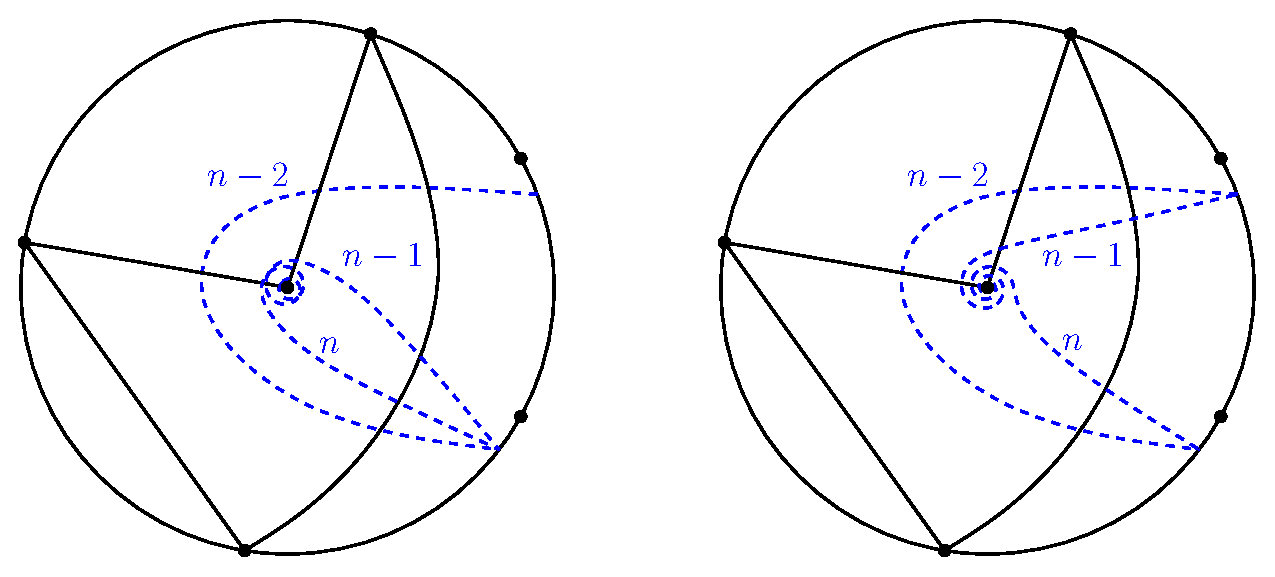
\includegraphics[scale=0.7]{D_n.eps}
    \end{center}
    \caption{ $D_n$.}
  \end{figure}


% bibliography
\bibliographystyle{amsalpha}
\bibliography{bibliography}

\end{document}
